% System structure: where the Draft Sequence and Post-Processing run and how
% the Draft/final images flow across the Android camera stack.
% Input directly from 2_1_draft_sequence.tex (Figure~\ref{fig:draft-arch}).
% Two-column float (figure*).
%
% Swimlanes (top->bottom): Application, Camera Framework, HAL, Storage.
% Loop: (1) the Camera App requests a capture down to the HAL; (2) the HAL
% returns frames & metadata up to the Framework; the Framework runs the
% Draft Sequence (fast, capture-critical) and the deferred Post-Processing;
% (3) the Draft image and (4) the final result are stored to the media DB;
% (5) the Gallery App shows the Draft image first and the final result once
% Post-Processing completes. Thumbnail glyphs match Fig.~\ref{fig:draft-pipeline}:
% flat gray Draft vs. portrait-bokeh final image.
\begin{figure*}[t]
  \centering
  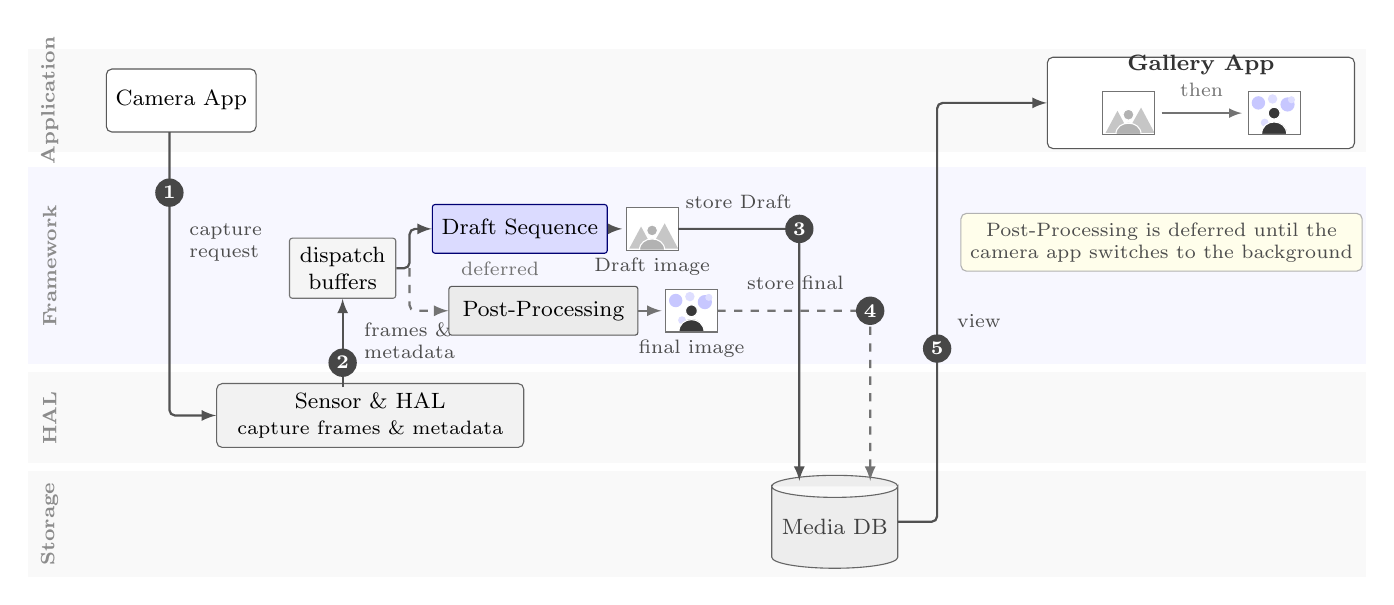
\begin{tikzpicture}[
    font=\footnotesize,
    >=latex,
    appbox/.style={draw=black!65, fill=white, rounded corners=2pt,
      align=center, minimum height=0.8cm},
    draftbox/.style={draw=blue!45!black, fill=blue!14, rounded corners=1pt,
      align=center, minimum height=0.62cm},
    finalbox/.style={draw=black!65, fill=gray!16, rounded corners=1pt,
      align=center, minimum height=0.62cm},
    plainbox/.style={draw=black!55, fill=gray!8, rounded corners=1pt,
      align=center},
    halbox/.style={draw=black!60, fill=gray!10, rounded corners=2pt,
      align=center},
    note/.style={draw=black!30, fill=yellow!8, rounded corners=2pt,
      align=center, font=\scriptsize, text=black!70},
    flow/.style={->, thick, black!68, rounded corners=2pt},
    defer/.style={->, thick, dashed, black!55, rounded corners=2pt},
    stepnum/.style={circle, fill=black!72, text=white, inner sep=0pt,
      minimum size=3.6mm, font=\scriptsize\bfseries},
    slabel/.style={text=black!70, font=\scriptsize},
    % ---- reusable thumbnail glyphs (local origin at bottom-left) ----
    draftpic/.pic={
      \fill[white] (0,0) rectangle (0.66,0.54);
      \fill[gray!45] (0.04,0.02) -- (0.19,0.30) -- (0.34,0.02) -- cycle;
      \fill[gray!45] (0.31,0.02) -- (0.49,0.34) -- (0.66,0.02) -- cycle;
      \draw[fill=gray!60, draw=white, line width=0.4pt]
        (0.17,0.0) .. controls (0.17,0.19) and (0.49,0.19) .. (0.49,0.0)
        -- cycle;
      \draw[fill=gray!60, draw=white, line width=0.4pt] (0.33,0.25)
        circle (0.07);
      \draw[black!55] (0,0) rectangle (0.66,0.54);
    },
    finalpic/.pic={
      \fill[white] (0,0) rectangle (0.66,0.54);
      \fill[blue!22] (0.13,0.40) circle (0.085);
      \fill[blue!13] (0.31,0.45) circle (0.06);
      \fill[blue!22] (0.50,0.38) circle (0.09);
      \fill[blue!13] (0.21,0.15) circle (0.05);
      \fill[blue!13] (0.55,0.44) circle (0.045);
      \draw[fill=black!78, draw=white, line width=0.4pt]
        (0.17,0.0) .. controls (0.17,0.21) and (0.49,0.21) .. (0.49,0.0)
        -- cycle;
      \draw[fill=black!78, draw=white, line width=0.4pt] (0.33,0.27)
        circle (0.075);
      \draw[black!55] (0,0) rectangle (0.66,0.54);
    }
  ]

    % ================= swimlane bands =================
    \fill[gray!5]  (0.2,5.70) rectangle (17.2,7.00);
    \fill[blue!3]  (0.2,3.00) rectangle (17.2,5.50);
    \fill[gray!5]  (0.2,1.75) rectangle (17.2,2.90);
    \fill[gray!5]  (0.2,0.30) rectangle (17.2,1.65);
    \node[rotate=90, text=black!45, font=\scriptsize\bfseries]
      at (0.48,6.35) {Application};
    \node[rotate=90, text=black!45, font=\scriptsize\bfseries]
      at (0.48,4.25) {Framework};
    \node[rotate=90, text=black!45, font=\scriptsize\bfseries]
      at (0.48,2.32) {HAL};
    \node[rotate=90, text=black!45, font=\scriptsize\bfseries]
      at (0.48,0.97) {Storage};

    % ================= Application: Camera App =================
    \node[appbox, minimum width=1.9cm] (capp) at (2.15,6.35) {Camera App};

    % ================= HAL =================
    \node[halbox, minimum width=3.9cm, minimum height=0.72cm]
      (hal) at (4.55,2.35) {Sensor \& HAL\\\scriptsize capture frames \& metadata};

    % (1) capture request : Camera App -> HAL
    \draw[flow] (2.0,5.95) -- (2.0,2.35) -- (hal.west);
    \node[anchor=west, align=left, slabel] at (2.13,4.55)
      {capture\\request};
    \node[stepnum] at (2.0,5.18) {1};

    % ================= Framework: dispatch + two paths =================
    \node[plainbox, minimum width=1.35cm, minimum height=0.72cm]
      (disp) at (4.2,4.22) {dispatch\\buffers};

    % (2) frames & metadata : HAL -> dispatch
    \draw[flow] (4.2,2.71) -- (disp.south);
    \node[anchor=west, align=left, slabel] at (4.35,3.30)
      {frames \&\\metadata};
    \node[stepnum] at (4.2,3.02) {2};

    \node[draftbox, minimum width=2.0cm] (ds) at (6.45,4.72)
      {Draft Sequence};
    \node[finalbox, minimum width=2.4cm] (pp) at (6.75,3.68)
      {Post-Processing};

    % fork dispatch -> Draft Sequence / Post-Processing
    \draw[flow] (disp.east) -- (5.05,4.22) |- (ds.west);
    \draw[defer] (5.05,4.22) |- (pp.west);
    \node[slabel, text=black!55, anchor=south] at (6.2,4.00) {deferred};

    % Draft Sequence -> Draft image thumbnail (fast)
    \draw[flow] (ds.east) -- (7.75,4.72);
    \pic at (7.80,4.45) {draftpic};
    \node[slabel] at (8.13,4.24) {Draft image};

    % Post-Processing -> final image thumbnail (deferred)
    \draw[defer] (pp.east) -- (8.25,3.68);
    \pic at (8.30,3.41) {finalpic};
    \node[slabel] at (8.63,3.20) {final image};

    % ================= Storage: media DB =================
    \draw[draw=black!60, fill=gray!14]
      (9.65,1.45) arc (180:360:0.8 and 0.14) -- (11.25,0.55)
      arc (0:-180:0.8 and 0.14) -- cycle;
    \draw[draw=black!60, fill=gray!14] (9.65,1.45) arc (180:0:0.8 and 0.14);
    \node[text=black!75] at (10.45,0.93) {Media DB};

    % (3) store Draft image (fast)
    \draw[flow] (8.46,4.72) -- (10.0,4.72) -- (10.0,1.52);
    \node[slabel, anchor=south] at (9.23,4.86) {store Draft};
    \node[stepnum] at (10.0,4.72) {3};

    % (4) store final result (deferred)
    \draw[defer] (8.96,3.68) -- (10.9,3.68) -- (10.9,1.52);
    \node[slabel, anchor=south] at (9.95,3.82) {store final};
    \node[stepnum] at (10.9,3.68) {4};

    % deferral note (placed in the otherwise-empty upper-right framework area)
    \node[note, minimum width=3.2cm] at (14.6,4.55)
      {Post-Processing is deferred until the\\camera app switches to the background};

    % ================= Application: Gallery App =================
    \node[appbox, minimum width=3.9cm, minimum height=1.16cm]
      (gapp) at (15.10,6.32) {};
    \node[text=black!80, font=\footnotesize\bfseries] at (15.10,6.80)
      {Gallery App};
    \pic at (13.85,5.92) {draftpic};
    \pic at (15.70,5.92) {finalpic};
    \draw[->, semithick, black!55] (14.60,6.19) -- (15.62,6.19);
    \node[slabel, text=black!55, anchor=south] at (15.11,6.28) {then};

    % (5) view : DB -> Gallery App (Draft first, final later)
    \draw[flow] (11.25,1.00) -- (11.75,1.00) -- (11.75,6.32) -- (gapp.west);
    \node[slabel, anchor=west] at (11.88,3.55) {view};
    \node[stepnum] at (11.75,3.20) {5};

  \end{tikzpicture}
  \caption{Where the Draft Sequence and Post-Processing run in the Android
  camera stack. (1)~The Camera App issues a capture request to the HAL, which
  (2)~returns frames and metadata to the Camera Framework. The Framework runs
  the Draft Sequence on the capture-critical path to produce the Draft image
  quickly, while heavy Post-Processing is deferred until the camera
  application switches to the background. (3)~The Draft image and (4)~the
  final result are stored to the media database, so that (5)~the Gallery App
  first shows the Draft image and later shows the final result once
  Post-Processing completes.}
  \label{fig:draft-arch}
\end{figure*}
